\documentclass[11pt]{article}

\newcommand{\titrechapitre}{Généralités sur les fonctions -- Exercices}
\newcommand{\titreclasse}{Lycée Jean-Baptiste \textsc{Corot}}
\newcommand{\pagination}{}%{\thepage/\pageref{LastPage}}
\newcommand{\topbotmargins}{1.5cm}
%%%%%%%%%%%%%%%%%%%%%%%%%%%%%%%%%%%%%%%%%%%%%%%%%%%%%%%%%%%%%%%%%%%%%%%%%%%%%%%%
%
% PACKAGES
% ========
%
%%%%%%%%%%%%%%%%%%%%%%%%%%%%%%%%%%%%%%%%%%%%%%%%%%%%%%%%%%%%%%%%%%%%%%%%%%%%%%%%

\usepackage[english, french]{babel}
\usepackage[utf8]{inputenc}
\usepackage[T1]{fontenc}
\usepackage{graphicx}
\usepackage{amsmath,amssymb,amsthm,amsopn}
\usepackage{hyperref}

% Pour avoir l'écriture \mathscr (math script)
% ============================================

\usepackage{mathrsfs}

% Deal with coma as a decimal separator
% =====================================

\usepackage{icomma}

% Package Geometry
% ================

\usepackage[a4paper, lmargin=2cm, rmargin=2cm, top=\topbotmargins, bottom=\topbotmargins]{geometry}

% Package multicol
% ================

\usepackage{multicol}

% Redefine abstract
% =================

% Note
% ====
%
% Le reste a été commenté pour ne pas charger trop de choses au démarrage. On
% verra si on en a besoin plus tard.
%
% --------
%
%\usepackage{mathrsfs}
%\usepackage{multirow}
%\usepackage{bm}
%\hypersetup{
%    colorlinks=true,
%    linkcolor=blue,
%    citecolor=red,
%}
%\usepackage{diagbox}
%
%\usepackage{algorithm}
%\usepackage{algpseudocode}
%
%\renewcommand{\algorithmicrequire}{\textbf{Input:}}
%\renewcommand{\algorithmicensure}{\textbf{Output:}}


%%%%%%%%%%%%%%%%%%%%%%%%%%%%%%%%%%%%%%%%%%%%%%%%%%%%%%%%%%%%%%%%%%%%%%%%%%%%%%%%
%
% TIKZ
% ====
%
%%%%%%%%%%%%%%%%%%%%%%%%%%%%%%%%%%%%%%%%%%%%%%%%%%%%%%%%%%%%%%%%%%%%%%%%%%%%%%%%

\usepackage{tikz}
\usetikzlibrary{arrows}

\usepackage{tkz-tab} % Variation tables

\usepackage{pgfplots}
%\usepackage{pgf-pie} % Pie charts

\pgfplotsset{
%\newcommand{\settingsgraph}{
x=.5cm,y=.5cm,
xticklabel style = {font=\scriptsize, yshift=.1cm},
yticklabel style = {font=\scriptsize, xshift=.1cm},
axis lines=middle,
ymajorgrids=true,
xmajorgrids=true,
major grid style = {color=white!80!blue},
xmin=-5.5,
xmax=5.5,
ymin=-5.5,
ymax=5.5,
xtick={-5.0,-4.0,...,5.0},
ytick={-5.0,-4.0,...,5.0},
}

% Tikz style

\tikzset{round/.style={circle, draw=black, very thick, scale = 0.7}}
\tikzset{arrow/.style={->, >=latex}}
\tikzset{dashed-arrow/.style={->, >=latex, dashed}}

\newcommand{\point}[3]{\draw[very thick, #3] (#1-.1, #2)--(#1+.1, #2)
(#1, #2-.1)--(#1, #2+.1)}

%%%%%%%%%%%%%%%%%%%%%%%%%%%%%%%%%%%%%%%%%%%%%%%%%%%%%%%%%%%%%%%%%%%%%%%%%%%%%%%%
%
% FANCY HEADER
% ============
%
%%%%%%%%%%%%%%%%%%%%%%%%%%%%%%%%%%%%%%%%%%%%%%%%%%%%%%%%%%%%%%%%%%%%%%%%%%%%%%%%


\usepackage{fancyhdr}
\usepackage{lastpage}

\pagestyle{fancy}
\newcommand{\changefont}{\fontsize{9}{9}\selectfont}
\renewcommand{\headrulewidth}{0mm}
\renewcommand{\footrulewidth}{0mm}

\fancyhead[C]{}
\fancyhead[L]{\titreclasse}
\fancyhead[R]{\titrechapitre}
\fancyfoot[C]{}
\fancyfoot[L]{}
\fancyfoot[R]{\pagination}
\addtolength{\skip\footins}{20pt} % distance between text and footnotes

%%%%%%%%%%%%%%%%%%%%%%%%%%%%%%%%%%%%%%%%%%%%%%%%%%%%%%%%%%%%%%%%%%%%%%%%%%%%%%%%
%
% THEOREM STYLE
% =============
%
%%%%%%%%%%%%%%%%%%%%%%%%%%%%%%%%%%%%%%%%%%%%%%%%%%%%%%%%%%%%%%%%%%%%%%%%%%%%%%%%

\usepackage[tikz]{bclogo}
\usepackage{mdframed}

\usepackage{tcolorbox}
\tcbuselibrary{listings, breakable, theorems, skins}

%\newtheoremstyle{break}%
%{}{}%
%{\itshape}{}%
%{\bfseries}{}%  % Note that final punctuation is omitted.
%{\newline}{}

\newtheoremstyle{scbf}%
{}{}%
{}{}%
%{\scshape}{}%  % Note that final punctuation is omitted.
{\bfseries\scshape}{}%  % Note that final punctuation is omitted.
{\newline}{}

%\theoremstyle{break}
%\theoremstyle{plain}
%\newtheorem{thm}{Theorem}[section]
%\newtheorem{lm}[thm]{Lemma}
%\newtheorem{prop}[thm]{Proposition}
%\newtheorem{cor}[thm]{Corollary}

%\theoremstyle{scbf}
%\newtheorem{exo}{$\star$ Exercice}

%\theoremstyle{definition}
%\newtheorem{defi}[thm]{Definition}
%\newtheorem{ex}[thm]{Example}

%\theoremstyle{remark}
%\newtheorem{rem}[thm]{Remark}

% Defining the Remark environment
% ===============================

\newenvironment{rmq}
  {
    \begin{bclogo}[logo=\bcinfo, noborder=true]{Remarque}
  }
  {
    \end{bclogo}
  }

% Defining the exercise environment
% =================================

\newcounter{exos}
\setcounter{exos}{1}

\newenvironment{exo}
  {
    \begin{bclogo}[logo=\bccrayon, noborder=true]{Exercice \theexos}
  }
  {
    \end{bclogo}
    \addtocounter{exos}{1}
  }


% Redefining the proof environment from amsthm
% ============================================

\tcolorboxenvironment{proof}{
  blanker, breakable, before skip=10pt,after skip=10pt,
  borderline west={1mm}{0pt}{red},
  left=5mm,
}

% Defining the definition environment
% ===================================

\colorlet{coldef}{black!50!green}

\newcounter{defis}
\setcounter{defis}{1}

\newenvironment{defi}[1]
  {
    \begin{defihid}{{#1}}{\thedefis}
  }
  {
    \end{defihid}
    \addtocounter{defis}{1}
  }

\newtcolorbox{defihid}[2]{%
  empty,title={ {\bfseries Définition {#2}} ({#1})},attach boxed title to top left,
boxed title style={empty,size=minimal,toprule=2pt,top=4pt,
overlay={\draw[coldef,line width=2pt]
([yshift=-1pt]frame.north west)--([yshift=-1pt]frame.north east);}},
coltitle=coldef,
before=\par\medskip\noindent,parbox=false,boxsep=0pt,left=0pt,right=3mm,top=4pt,
breakable,pad at break*=0mm,vfill before first,
overlay unbroken={\draw[coldef,line width=1pt]
([yshift=-1pt]title.north east)--([xshift=-0.5pt,yshift=-1pt]title.north-|frame.east)
--([xshift=-0.5pt]frame.south east)--(frame.south west); },
overlay first={\draw[coldef,line width=1pt]
([yshift=-1pt]title.north east)--([xshift=-0.5pt,yshift=-1pt]title.north-|frame.east)
--([xshift=-0.5pt]frame.south east); },
overlay middle={\draw[coldef,line width=1pt] ([xshift=-0.5pt]frame.north east)
--([xshift=-0.5pt]frame.south east); },
overlay last={\draw[coldef,line width=1pt] ([xshift=-0.5pt]frame.north east)
--([xshift=-0.5pt]frame.south east)--(frame.south west);},%
}

\newenvironment{notation}
  {
    \begin{notationhid}{\thedefis}
  }
  {
    \end{notationhid}
    \addtocounter{defis}{1}
  }

\newtcolorbox{notationhid}[1]{%
  empty,title={Notation {#1}},attach boxed title to top left,
boxed title style={empty,size=minimal,toprule=2pt,top=4pt,
overlay={\draw[coldef,line width=2pt]
([yshift=-1pt]frame.north west)--([yshift=-1pt]frame.north east);}},
coltitle=coldef,fonttitle=\bfseries,
before=\par\medskip\noindent,parbox=false,boxsep=0pt,left=0pt,right=3mm,top=4pt,
breakable,pad at break*=0mm,vfill before first,
overlay unbroken={\draw[coldef,line width=1pt]
([yshift=-1pt]title.north east)--([xshift=-0.5pt,yshift=-1pt]title.north-|frame.east)
--([xshift=-0.5pt]frame.south east)--(frame.south west); },
overlay first={\draw[coldef,line width=1pt]
([yshift=-1pt]title.north east)--([xshift=-0.5pt,yshift=-1pt]title.north-|frame.east)
--([xshift=-0.5pt]frame.south east); },
overlay middle={\draw[coldef,line width=1pt] ([xshift=-0.5pt]frame.north east)
--([xshift=-0.5pt]frame.south east); },
overlay last={\draw[coldef,line width=1pt] ([xshift=-0.5pt]frame.north east)
--([xshift=-0.5pt]frame.south east)--(frame.south west);},%
}


% Defining the proposition, theorem, etc. environment
% ===================================================

\colorlet{colprop}{red!75!black}

\newcounter{props}
\setcounter{props}{1}

\newenvironment{prop}
  {
    \begin{prophid}{\theprops}
  }
  {
    \end{prophid}
    \refstepcounter{props}
  }

\newtcolorbox{prophid}[1]{%
empty,title={Propriété {#1}},attach boxed title to top left,
boxed title style={empty,size=minimal,toprule=2pt,top=4pt,
overlay={\draw[colprop,line width=2pt]
([yshift=-1pt]frame.north west)--([yshift=-1pt]frame.north east);}},
coltitle=colprop,fonttitle=\bfseries,
before=\par\medskip\noindent,parbox=false,boxsep=0pt,left=0pt,right=3mm,top=4pt,
breakable,pad at break*=0mm,vfill before first,
overlay unbroken={\draw[colprop,line width=1pt]
([yshift=-1pt]title.north east)--([xshift=-0.5pt,yshift=-1pt]title.north-|frame.east)
--([xshift=-0.5pt]frame.south east)--(frame.south west); },
overlay first={\draw[colprop,line width=1pt]
([yshift=-1pt]title.north east)--([xshift=-0.5pt,yshift=-1pt]title.north-|frame.east)
--([xshift=-0.5pt]frame.south east); },
overlay middle={\draw[colprop,line width=1pt] ([xshift=-0.5pt]frame.north east)
--([xshift=-0.5pt]frame.south east); },
overlay last={\draw[colprop,line width=1pt] ([xshift=-0.5pt]frame.north east)
--([xshift=-0.5pt]frame.south east)--(frame.south west);},%
}

\newenvironment{propadm}
  {
    \begin{propadmhid}{\theprops}
  }
  {
    \end{propadmhid}
    \refstepcounter{props}
  }

  \newtcolorbox{propadmhid}[1]{%
    empty,title={{\bfseries Propriété {#1}} (admise)},attach boxed title to top left,
boxed title style={empty,size=minimal,toprule=2pt,top=4pt,
overlay={\draw[colprop,line width=2pt]
([yshift=-1pt]frame.north west)--([yshift=-1pt]frame.north east);}},
coltitle=colprop,%fonttitle=\bfseries,
before=\par\medskip\noindent,parbox=false,boxsep=0pt,left=0pt,right=3mm,top=4pt,
breakable,pad at break*=0mm,vfill before first,
overlay unbroken={\draw[colprop,line width=1pt]
([yshift=-1pt]title.north east)--([xshift=-0.5pt,yshift=-1pt]title.north-|frame.east)
--([xshift=-0.5pt]frame.south east)--(frame.south west); },
overlay first={\draw[colprop,line width=1pt]
([yshift=-1pt]title.north east)--([xshift=-0.5pt,yshift=-1pt]title.north-|frame.east)
--([xshift=-0.5pt]frame.south east); },
overlay middle={\draw[colprop,line width=1pt] ([xshift=-0.5pt]frame.north east)
--([xshift=-0.5pt]frame.south east); },
overlay last={\draw[colprop,line width=1pt] ([xshift=-0.5pt]frame.north east)
--([xshift=-0.5pt]frame.south east)--(frame.south west);},%
}

\newenvironment{propnom}[1]
  {
    \begin{propnomhid}{#1}{\theprops}
  }
  {
    \end{propnomhid}
    \refstepcounter{props}
  }

\newtcolorbox{propnomhid}[2]{%
empty,title={{\bfseries Propriété {#2}} ({#1})},attach boxed title to top left,
boxed title style={empty,size=minimal,toprule=2pt,top=4pt,
overlay={\draw[colprop,line width=2pt]
([yshift=-1pt]frame.north west)--([yshift=-1pt]frame.north east);}},
coltitle=colprop,
before=\par\medskip\noindent,parbox=false,boxsep=0pt,left=0pt,right=3mm,top=4pt,
breakable,pad at break*=0mm,vfill before first,
overlay unbroken={\draw[colprop,line width=1pt]
([yshift=-1pt]title.north east)--([xshift=-0.5pt,yshift=-1pt]title.north-|frame.east)
--([xshift=-0.5pt]frame.south east)--(frame.south west); },
overlay first={\draw[colprop,line width=1pt]
([yshift=-1pt]title.north east)--([xshift=-0.5pt,yshift=-1pt]title.north-|frame.east)
--([xshift=-0.5pt]frame.south east); },
overlay middle={\draw[colprop,line width=1pt] ([xshift=-0.5pt]frame.north east)
--([xshift=-0.5pt]frame.south east); },
overlay last={\draw[colprop,line width=1pt] ([xshift=-0.5pt]frame.north east)
--([xshift=-0.5pt]frame.south east)--(frame.south west);},%
}




\newenvironment{thm}
  {
    \begin{thmhid}{\theprops}
  }
  {
    \end{thmhid}
    \refstepcounter{props}
  }

\newtcolorbox{thmhid}[1]{%
empty,title={Théorème {#1}},attach boxed title to top left,
boxed title style={empty,size=minimal,toprule=2pt,top=4pt,
overlay={\draw[colprop,line width=2pt]
([yshift=-1pt]frame.north west)--([yshift=-1pt]frame.north east);}},
coltitle=colprop,fonttitle=\bfseries,
before=\par\medskip\noindent,parbox=false,boxsep=0pt,left=0pt,right=3mm,top=4pt,
breakable,pad at break*=0mm,vfill before first,
overlay unbroken={\draw[colprop,line width=1pt]
([yshift=-1pt]title.north east)--([xshift=-0.5pt,yshift=-1pt]title.north-|frame.east)
--([xshift=-0.5pt]frame.south east)--(frame.south west); },
overlay first={\draw[colprop,line width=1pt]
([yshift=-1pt]title.north east)--([xshift=-0.5pt,yshift=-1pt]title.north-|frame.east)
--([xshift=-0.5pt]frame.south east); },
overlay middle={\draw[colprop,line width=1pt] ([xshift=-0.5pt]frame.north east)
--([xshift=-0.5pt]frame.south east); },
overlay last={\draw[colprop,line width=1pt] ([xshift=-0.5pt]frame.north east)
--([xshift=-0.5pt]frame.south east)--(frame.south west);},%
}

\newenvironment{thmadm}
  {
    \begin{thmadmhid}{\theprops}
  }
  {
    \end{thmadmhid}
    \refstepcounter{props}
  }

  \newtcolorbox{thmadmhid}[1]{%
    empty,title={{\bfseries Théorème {#1}} (admis)},attach boxed title to top left,
boxed title style={empty,size=minimal,toprule=2pt,top=4pt,
overlay={\draw[colprop,line width=2pt]
([yshift=-1pt]frame.north west)--([yshift=-1pt]frame.north east);}},
coltitle=colprop,%fonttitle=\bfseries,
before=\par\medskip\noindent,parbox=false,boxsep=0pt,left=0pt,right=3mm,top=4pt,
breakable,pad at break*=0mm,vfill before first,
overlay unbroken={\draw[colprop,line width=1pt]
([yshift=-1pt]title.north east)--([xshift=-0.5pt,yshift=-1pt]title.north-|frame.east)
--([xshift=-0.5pt]frame.south east)--(frame.south west); },
overlay first={\draw[colprop,line width=1pt]
([yshift=-1pt]title.north east)--([xshift=-0.5pt,yshift=-1pt]title.north-|frame.east)
--([xshift=-0.5pt]frame.south east); },
overlay middle={\draw[colprop,line width=1pt] ([xshift=-0.5pt]frame.north east)
--([xshift=-0.5pt]frame.south east); },
overlay last={\draw[colprop,line width=1pt] ([xshift=-0.5pt]frame.north east)
--([xshift=-0.5pt]frame.south east)--(frame.south west);},%
}

\newenvironment{thmnom}[1]
  {
    \begin{thmnomhid}{#1}{\theprops}
  }
  {
    \end{thmnomhid}
    \refstepcounter{props}
  }

\newtcolorbox{thmnomhid}[2]{%
empty,title={{\bfseries Théorème {#2}} ({#1})},attach boxed title to top left,
boxed title style={empty,size=minimal,toprule=2pt,top=4pt,
overlay={\draw[colprop,line width=2pt]
([yshift=-1pt]frame.north west)--([yshift=-1pt]frame.north east);}},
coltitle=colprop,
before=\par\medskip\noindent,parbox=false,boxsep=0pt,left=0pt,right=3mm,top=4pt,
breakable,pad at break*=0mm,vfill before first,
overlay unbroken={\draw[colprop,line width=1pt]
([yshift=-1pt]title.north east)--([xshift=-0.5pt,yshift=-1pt]title.north-|frame.east)
--([xshift=-0.5pt]frame.south east)--(frame.south west); },
overlay first={\draw[colprop,line width=1pt]
([yshift=-1pt]title.north east)--([xshift=-0.5pt,yshift=-1pt]title.north-|frame.east)
--([xshift=-0.5pt]frame.south east); },
overlay middle={\draw[colprop,line width=1pt] ([xshift=-0.5pt]frame.north east)
--([xshift=-0.5pt]frame.south east); },
overlay last={\draw[colprop,line width=1pt] ([xshift=-0.5pt]frame.north east)
--([xshift=-0.5pt]frame.south east)--(frame.south west);},%
}

\newenvironment{coro}
  {
    \begin{corohid}{\theprops}
  }
  {
    \end{corohid}
    \refstepcounter{props}
  }

  \newtcolorbox{corohid}[1]{%
  empty,title={Corollaire {#1}},attach boxed title to top left,
boxed title style={empty,size=minimal,toprule=2pt,top=4pt,
overlay={\draw[colprop,line width=2pt]
([yshift=-1pt]frame.north west)--([yshift=-1pt]frame.north east);}},
coltitle=colprop,fonttitle=\bfseries,
before=\par\medskip\noindent,parbox=false,boxsep=0pt,left=0pt,right=3mm,top=4pt,
breakable,pad at break*=0mm,vfill before first,
overlay unbroken={\draw[colprop,line width=1pt]
([yshift=-1pt]title.north east)--([xshift=-0.5pt,yshift=-1pt]title.north-|frame.east)
--([xshift=-0.5pt]frame.south east)--(frame.south west); },
overlay first={\draw[colprop,line width=1pt]
([yshift=-1pt]title.north east)--([xshift=-0.5pt,yshift=-1pt]title.north-|frame.east)
--([xshift=-0.5pt]frame.south east); },
overlay middle={\draw[colprop,line width=1pt] ([xshift=-0.5pt]frame.north east)
--([xshift=-0.5pt]frame.south east); },
overlay last={\draw[colprop,line width=1pt] ([xshift=-0.5pt]frame.north east)
--([xshift=-0.5pt]frame.south east)--(frame.south west);},%
}

\newenvironment{lemme}
  {
    \begin{lemmehid}{\theprops}
  }
  {
    \end{lemmehid}
    \refstepcounter{props}
  }

  \newtcolorbox{lemmehid}[1]{%
  empty,title={Lemme {#1}},attach boxed title to top left,
boxed title style={empty,size=minimal,toprule=2pt,top=4pt,
overlay={\draw[colprop,line width=2pt]
([yshift=-1pt]frame.north west)--([yshift=-1pt]frame.north east);}},
coltitle=colprop,fonttitle=\bfseries,
before=\par\medskip\noindent,parbox=false,boxsep=0pt,left=0pt,right=3mm,top=4pt,
breakable,pad at break*=0mm,vfill before first,
overlay unbroken={\draw[colprop,line width=1pt]
([yshift=-1pt]title.north east)--([xshift=-0.5pt,yshift=-1pt]title.north-|frame.east)
--([xshift=-0.5pt]frame.south east)--(frame.south west); },
overlay first={\draw[colprop,line width=1pt]
([yshift=-1pt]title.north east)--([xshift=-0.5pt,yshift=-1pt]title.north-|frame.east)
--([xshift=-0.5pt]frame.south east); },
overlay middle={\draw[colprop,line width=1pt] ([xshift=-0.5pt]frame.north east)
--([xshift=-0.5pt]frame.south east); },
overlay last={\draw[colprop,line width=1pt] ([xshift=-0.5pt]frame.north east)
--([xshift=-0.5pt]frame.south east)--(frame.south west);},%
}

\colorlet{colexemple}{blue!50!black}
%\newtcolorbox{exemple}{empty, title=Exemple, attach boxed title to top left,
%  boxed title style={empty, size=minimal, toprule=2pt, top=4pt,
%    overlay={\draw[colexemple,line width=2pt]
%([yshift=-1pt]frame.north west)--([yshift=-1pt]frame.north east);}},
%coltitle=colexemple,fonttitle=\bfseries,%\large\bfseries,
%before=\par\medskip\noindent,parbox=false,boxsep=0pt,left=0pt,right=3mm,top=4pt,
%overlay={\draw[colexemple,line width=1pt]
%([yshift=-1pt]title.north east)--([xshift=-0.5pt,yshift=-1pt]title.north-|frame.east)
%--([xshift=-0.5pt]frame.south east)--(frame.south west); },
%}

\newcounter{exemples}
\setcounter{exemples}{1}

\newenvironment{exemple}
  {
    \begin{exemplehid}{\theexemples}
  }
  {
    \end{exemplehid}
    \addtocounter{exemples}{1}
  }

\newtcolorbox{exemplehid}[1]{%
empty,title={Exemple {#1}},attach boxed title to top left,
boxed title style={empty,size=minimal,toprule=2pt,top=4pt,
overlay={\draw[colexemple,line width=2pt]
([yshift=-1pt]frame.north west)--([yshift=-1pt]frame.north east);}},
coltitle=colexemple,fonttitle=\bfseries,
before=\par\medskip\noindent,parbox=false,boxsep=0pt,left=0pt,right=3mm,top=4pt,
breakable,pad at break*=0mm,vfill before first,
overlay unbroken={\draw[colexemple,line width=1pt]
([yshift=-1pt]title.north east)--([xshift=-0.5pt,yshift=-1pt]title.north-|frame.east)
--([xshift=-0.5pt]frame.south east)--(frame.south west); },
overlay first={\draw[colexemple,line width=1pt]
([yshift=-1pt]title.north east)--([xshift=-0.5pt,yshift=-1pt]title.north-|frame.east)
--([xshift=-0.5pt]frame.south east); },
overlay middle={\draw[colexemple,line width=1pt] ([xshift=-0.5pt]frame.north east)
--([xshift=-0.5pt]frame.south east); },
overlay last={\draw[colexemple,line width=1pt] ([xshift=-0.5pt]frame.north east)
--([xshift=-0.5pt]frame.south east)--(frame.south west);},%
}

\newenvironment{contrex}
  {
    \begin{contrexhid}{\theexemples}
  }
  {
    \end{contrexhid}
    \addtocounter{exemples}{1}
  }

\newtcolorbox{contrexhid}[1]{%
empty,title={Contre-exemple {#1}},attach boxed title to top left,
boxed title style={empty,size=minimal,toprule=2pt,top=4pt,
overlay={\draw[colexemple,line width=2pt]
([yshift=-1pt]frame.north west)--([yshift=-1pt]frame.north east);}},
coltitle=colexemple,fonttitle=\bfseries,
before=\par\medskip\noindent,parbox=false,boxsep=0pt,left=0pt,right=3mm,top=4pt,
breakable,pad at break*=0mm,vfill before first,
overlay unbroken={\draw[colexemple,line width=1pt]
([yshift=-1pt]title.north east)--([xshift=-0.5pt,yshift=-1pt]title.north-|frame.east)
--([xshift=-0.5pt]frame.south east)--(frame.south west); },
overlay first={\draw[colexemple,line width=1pt]
([yshift=-1pt]title.north east)--([xshift=-0.5pt,yshift=-1pt]title.north-|frame.east)
--([xshift=-0.5pt]frame.south east); },
overlay middle={\draw[colexemple,line width=1pt] ([xshift=-0.5pt]frame.north east)
--([xshift=-0.5pt]frame.south east); },
overlay last={\draw[colexemple,line width=1pt] ([xshift=-0.5pt]frame.north east)
--([xshift=-0.5pt]frame.south east)--(frame.south west);},%
}

\newenvironment{app}
  {
    \begin{apphid}{\theexemples}
  }
  {
    \end{apphid}
    \addtocounter{exemples}{1}
  }

\newtcolorbox{apphid}[1]{%
empty,title={Application {#1}},attach boxed title to top left,
boxed title style={empty,size=minimal,toprule=2pt,top=4pt,
overlay={\draw[colexemple,line width=2pt]
([yshift=-1pt]frame.north west)--([yshift=-1pt]frame.north east);}},
coltitle=colexemple,fonttitle=\bfseries,
before=\par\medskip\noindent,parbox=false,boxsep=0pt,left=0pt,right=3mm,top=4pt,
breakable,pad at break*=0mm,vfill before first,
overlay unbroken={\draw[colexemple,line width=1pt]
([yshift=-1pt]title.north east)--([xshift=-0.5pt,yshift=-1pt]title.north-|frame.east)
--([xshift=-0.5pt]frame.south east)--(frame.south west); },
overlay first={\draw[colexemple,line width=1pt]
([yshift=-1pt]title.north east)--([xshift=-0.5pt,yshift=-1pt]title.north-|frame.east)
--([xshift=-0.5pt]frame.south east); },
overlay middle={\draw[colexemple,line width=1pt] ([xshift=-0.5pt]frame.north east)
--([xshift=-0.5pt]frame.south east); },
overlay last={\draw[colexemple,line width=1pt] ([xshift=-0.5pt]frame.north east)
--([xshift=-0.5pt]frame.south east)--(frame.south west);},%
}

%%%%%%%%%%%%%%%%%%%%%%%%%%%%%%%%%%%%%%%%%%%%%%%%%%%%%%%%%%%%%%%%%%%%%%%%%%%%%%%%
%
% ENUMERATE
% =========
%
%%%%%%%%%%%%%%%%%%%%%%%%%%%%%%%%%%%%%%%%%%%%%%%%%%%%%%%%%%%%%%%%%%%%%%%%%%%%%%%%

\usepackage{enumerate}
\usepackage{enumitem}

% To have special enumerate items like
%
% 1/
% 2/
% 3/

%%%%%%%%%%%%%%%%%%%%%%%%%%%%%%%%%%%%%%%%%%%%%%%%%%%%%%%%%%%%%%%%%%%%%%%%%%%%%%%%
%
% ARRAYS
% ======
%
%%%%%%%%%%%%%%%%%%%%%%%%%%%%%%%%%%%%%%%%%%%%%%%%%%%%%%%%%%%%%%%%%%%%%%%%%%%%%%%%


\usepackage{array}
\usepackage{makecell} % Used to break lines within arrays
\usepackage{multirow}
\usepackage{booktabs} % Used to have nice arrays with headrules

%%%%%%%%%%%%%%%%%%%%%%%%%%%%%%%%%%%%%%%%%%%%%%%%%%%%%%%%%%%%%%%%%%%%%%%%%%%%%%%%
%
% WRITE CODE
% ==========
%
%%%%%%%%%%%%%%%%%%%%%%%%%%%%%%%%%%%%%%%%%%%%%%%%%%%%%%%%%%%%%%%%%%%%%%%%%%%%%%%%

\usepackage{listings}
\usepackage{xcolor}

%New colors defined below
\definecolor{codegreen}{rgb}{0,0.6,0}
\definecolor{codegray}{rgb}{0.5,0.5,0.5}
\definecolor{codepurple}{rgb}{0.58,0,0.82}
\definecolor{backcolour}{rgb}{0.95,0.95,0.92}

%Code listing style named "mystyle"
\lstdefinestyle{python}{
  %backgroundcolor=\color{backcolour},
  commentstyle=\color{codegreen},
  keywordstyle=\color{magenta},
  numberstyle=\tiny\color{codegray},
  stringstyle=\color{codepurple},
  basicstyle=\ttfamily\footnotesize,
  breakatwhitespace=false,
  breaklines=true,
  captionpos=b,
  keepspaces=true,
  numbers=left,
  numbersep=5pt,
  showspaces=false,
  showstringspaces=false,
  showtabs=false,
  tabsize=2
}

\lstset{style=python}

%%%%%%%%%%%%%%%%%%%%%%%%%%%%%%%%%%%%%%%%%%%%%%%%%%%%%%%%%%%%%%%%%%%%%%%%%%%%%%%%
%
% Tabular 
% =======
%
%%%%%%%%%%%%%%%%%%%%%%%%%%%%%%%%%%%%%%%%%%%%%%%%%%%%%%%%%%%%%%%%%%%%%%%%%%%%%%%%

% In order to obtain a tabular with given width.

\usepackage{tabularx}
\newcolumntype{Y}{>{\centering\arraybackslash}X}
\newcolumntype{R}{>{\raggedright\arraybackslash}X}
\newcolumntype{L}{>{\raggedleft\arraybackslash}X}
% \usepackage{tabulary} % younger brother

%%%%%%%%%%%%%%%%%%%%%%%%%%%%%%%%%%%%%%%%%%%%%%%%%%%%%%%%%%%%%%%%%%%%%%%%%%%%%%%%
%
% MACROS
% ======
%
%%%%%%%%%%%%%%%%%%%%%%%%%%%%%%%%%%%%%%%%%%%%%%%%%%%%%%%%%%%%%%%%%%%%%%%%%%%%%%%%

% Math Operators

\DeclareMathOperator{\Card}{Card}
\DeclareMathOperator{\Gal}{Gal}
\DeclareMathOperator{\Id}{Id}
\DeclareMathOperator{\Img}{Im}
\DeclareMathOperator{\Ker}{Ker}
\DeclareMathOperator{\Minpoly}{Minpoly}
\DeclareMathOperator{\Mod}{mod}
\DeclareMathOperator{\Ord}{Ord}
\DeclareMathOperator{\ppcm}{ppcm}
\DeclareMathOperator{\pgcd}{pgcd}
\DeclareMathOperator{\tr}{Tr}
\DeclareMathOperator{\Vect}{Vect}
\DeclareMathOperator{\Span}{Span}
\DeclareMathOperator{\rank}{rank}
\DeclareMathOperator{\rg}{rg}
\DeclareMathOperator{\ev}{ev}
\DeclareMathOperator{\Var}{Var}

% Shortcuts

\newcommand{\eg}{\emph{e.g. }}
\newcommand{\ent}[2]{[\![#1,#2]\!]}
\newcommand{\ie}{\emph{i.e. }}
\newcommand{\ps}[2]{\left\langle#1,#2\right\rangle}
\newcommand{\eqdef}{\overset{\text{def}}{=}}
\newcommand{\E}{\mathcal{E}}
\newcommand{\M}{\mathcal{M}}
\newcommand{\A}{\mathcal{A}}
\newcommand{\B}{\mathcal{B}}
\newcommand{\R}{\mathcal{R}}
\newcommand{\D}{\mathcal{D}}
\newcommand{\Pcal}{\mathcal{P}}
\newcommand{\K}{\mathbf{k}}
\newcommand{\vect}[1]{\overrightarrow{#1}}


%\input{layout-nb.tex}

\newcommand{\Cf}{\mathscr{C}_f}
\newcommand{\Cg}{\mathscr{C}_g}

\title{Chapitre 5 : Généralités sur les fonctions}
\date{}
\author{}

\begin{document}
%\maketitle\thispagestyle{fancy}

\paragraph{Exercice 1.} On considère la fonction $f$ définie sur $[-3;3]$ par
$f(x)=x^2$.
\begin{enumerate}
  \item À l'aide de la calculatrice, obtenir un tableau de valeurs, en partant
    de $-3$, avec un pas de $1$.
  \item Tracer la courbe représentative de $f$ dans un repère orthonormé.
\end{enumerate}

\paragraph{Exercice 2.} On considère la fonction $f$ définie sur $[-4;4]$ par
$f(x)=\frac{x^3}{10}$.
\begin{enumerate}
  \item À l'aide de la calculatrice, obtenir un tableau de valeurs, en partant
    de $-4$, avec un pas de $1$.
  \item Tracer la courbe représentative de $f$ dans un repère orthonormé.
\end{enumerate}

\paragraph{Exercice 3.} On considère une fonction $f$ vérifiant $f(2)=3$.
Compléter les phrases à trous suivantes.
\begin{enumerate}
  \item $\dots\dots\dots$ a pour image $\dots\dots\dots$ par la fonction $f$.
  \item Le point $A(\dots;\dots)$ est un point de la courbe représentative de la
    fonction $f$.
  \item Le nombre réel $\dots\dots$ est une solution de l'équation
    $f(x)=\dots\dots$.
  \item Le nombre réel $\dots\dots$ est un antécédent de $\dots\dots$ par la
    fonction $f$.
\end{enumerate}

\paragraph{Exercice 4.} Les vétérinaires donnent parfois le tableau de
correspondance entre l'\^age des chats et 
\begin{minipage}[]{.4\textwidth}
l'équivalent en \^age humain ci-contre. On note $c$ l'\^age du chat en année et
$H(c)$ l'\^age humain en équivalent en année.
\end{minipage}
\begin{minipage}{.6\textwidth}
\begin{center}
\begin{tabular}{ccccccc}
  \toprule
  \textbf{\^Age du chat (en année)} & $0,5$ & $1$ & $2$ & $6$ & $12$ & $16$ \\
  \midrule
  \textbf{\^Age humain (en année)} & $10$ & $18$ & $26$ & $42$ & $70$ & $94$ \\
  \bottomrule
\end{tabular}
  \end{center}
\end{minipage}
\begin{enumerate}
  \item Dans un repère orthogonal, tracer une courbe représentant la fonction
    $H$ sur $[0;16]$.
  \item Les deux \^ages sont-ils proportionnels ? Justifier.\\\emph{Quelle est
    la représentation graphique qui modélise une situation de proportionnalité ?}
  \item Préciser l'image de $3$ et interpréter la réponse.
  \item Donner un antécédent de $60$ et interpréter la réponse.
\end{enumerate}

\paragraph{Exercice 5.}~\\
\begin{minipage}{.6\textwidth}
Dans un repère orthogonal, on a tracé la représentation
graphique d'une fonction $f$.
  \begin{enumerate}
    \item Déterminer l'ensemble de définition $D_f$.
    \item Donner l'image de $-4$ par la fonction $f$.
    \item Donner $f(-2)$, $f(3)$ et $f(4)$.
    \item Quels sont les antécédents de $5$ par $f$ ? De $-1$ ? De $0$ ?
  \end{enumerate}
\end{minipage}
\begin{minipage}{.4\textwidth}
  \begin{center}
    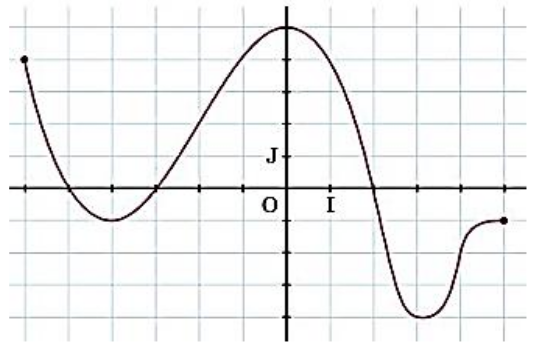
\includegraphics[scale=.3]{graph.png}
  \end{center}
\end{minipage}

\paragraph{Exercice 6.}~\\[-3mm]
\begin{minipage}{.5\textwidth}
  On considère les trois verres ci-contre et on note $h$ la hauteur du liquide
  contenu dans chaque verre. On note $V_1(h)$, $V_2(h)$ et $V_3(h)$ les volumes
  respectifs de liquide (en cL) dans ces $3$ verres en fonction de $h$ (en cm)
  jusqu'à remplissage complet.
\end{minipage}
\begin{minipage}{.5\textwidth}
  \begin{center}
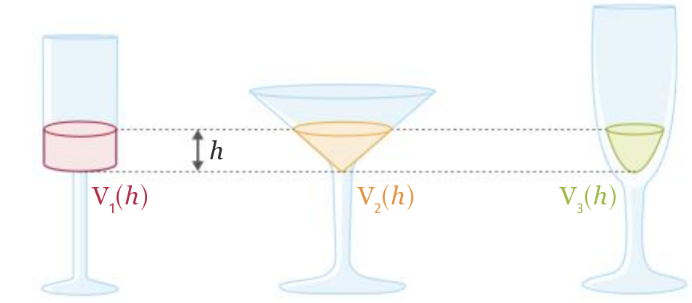
\includegraphics[scale=.3]{verres.png}
  \end{center}
\end{minipage}
\begin{minipage}{.65\textwidth}
  On a tracé ci-contre les différentes courbes représentatives des fonctions
  $V_1$, $V_2$ et $V_3$. Pour chacun des trois verres :
  \begin{enumerate}
    \item Préciser les ensembles de définition des volumes associés ainsi que
      les images à leurs extrémités. Interpréter ces résultats.
    \item Préciser le volume à mi-hauteur, puis la hauteur du verre quand il est
      à moitié plein.
    \item On verse $20$ cL : préciser la hauteur du liquide dans chacun des
      trois verres.
    \item Déterminer les coordonnées des différents points d'intersection et
      interpréter le résultat.
  \end{enumerate}
\end{minipage}
\begin{minipage}{.35\textwidth}
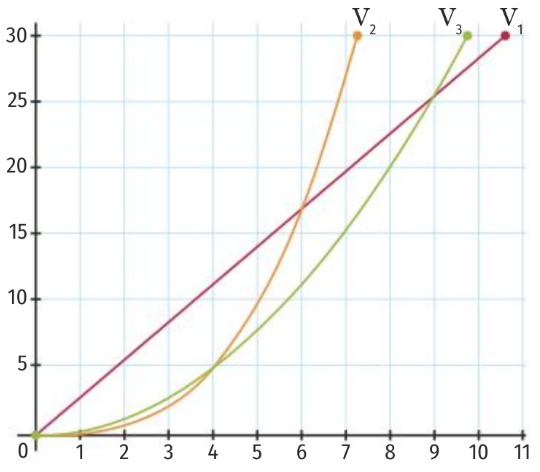
\includegraphics[scale=.3]{graph-verres.png}
\end{minipage}
\begin{enumerate}
    \setcounter{enumi}{4}
  \item Si on remplit les trois verres à une même hauteur, est-il possible que
    les trois convives aient le même volume de liquide ? Justifier.
\end{enumerate}

\paragraph{Exercice 7.} La fonction $f$ est représentée par la courbe
$\mathscr{C}_f$. Compléter le tableau suivant.
\begin{center}
  \def\arraystretch{2}
  \begin{tabular}{|c|c|c|}
    \hline
    \textbf{Images ou antécédents} & $f(x)=y$ & \textbf{Courbe} $\mathscr C_f$\\
    \hline
    $3$ a pour image $-1$ par $f$ & & \\
    \hline
    & $f(2)=5$ & \\
    \hline
    & & $A(1;-2)\in\mathscr C_f$ \\
    \hline
    $0$ est un antécédent de $4$ par $f$ & & \\
    \hline
    & & $B(5;12)\in\mathscr C_f$ \\
    \hline
    $8$ a pour antécédents $-1$ et $9$ par $f$ & & \\
    \hline
  \end{tabular}
\end{center}

\paragraph{Exercice 8.}
\begin{enumerate}
  \item Soit $\mathscr C_f$ la courbe représentative de la fonction $f$ définie
    sur $\mathbb{R}$ par $f(x)=\sqrt{25-x^2}$.
    \begin{enumerate}
      \item Le point $(-4;3)$ appartient-il à la courbe $\mathscr C_f$ ?
        Justifier.
      \item Même question avec le point $\left( \frac{1}{2};\frac{9}{2}
        \right)$.
    \end{enumerate}
  \item Soit $\mathscr C_g$ la courbe représentative de la fonction $g$ définie
    sur $\mathbb{R}$ par $g(x) = \frac{5x-4}{2}$.\\
    Le point $(6; 13)$ appartient-il à la courbe $\mathscr C_f$ ? Justifier.
\end{enumerate}

\paragraph{Exercice 9.}~\\
\begin{minipage}{.5\textwidth}
  Dans chaque cas, on a représenté dans un repère orthonormé une fonction $f$
  définie sur $\mathbb{R}$. Pour chacune d'elle
  \begin{enumerate}
    \item préciser graphiquement les solitions des équations $f(x)=-0,5$;
      $f(x)=0$ et $f(x)=2$;
    \item déterminer, suivant les valeurs de $k$, le nombre de solutions de
      l'équation $f(x)=k$ où $k\in\mathbb{R}$.
  \end{enumerate}
\end{minipage}
\begin{minipage}{.5\textwidth}
  \begin{center}
    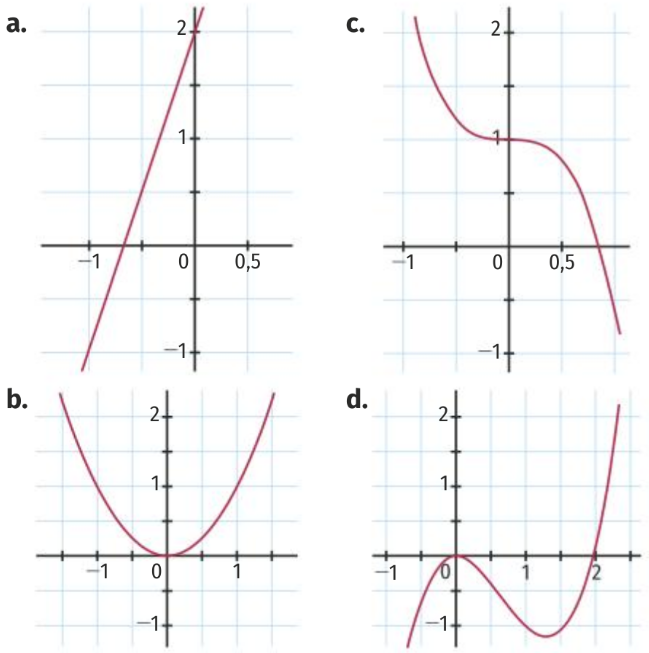
\includegraphics[scale=.3]{4fonctions.png}
  \end{center}
\end{minipage}

\paragraph{Exercice 10.}~\\[2mm]
\begin{minipage}{.5\textwidth}
  On considère la hauteur $H$, en mètre, d'un type d'arbre en fonction de son
  \^age $t$ (en mois).
  \begin{enumerate}
    \item Déterminer et interpréter $H(1)$.
    \item Ces arbres sont commercialisables dès qu'ils mesurent au moins $2$ m :
      traduire cela par une inéquation et la résoudre.
  \end{enumerate}
\end{minipage}
\begin{minipage}{.5\textwidth}
  \begin{center}
    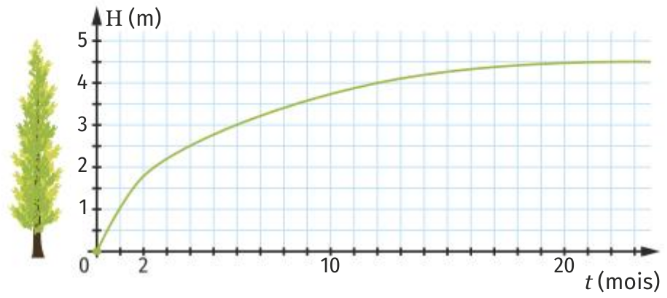
\includegraphics[scale=.35]{arbres.png}
  \end{center}
\end{minipage}
\begin{enumerate}
    \setcounter{enumi}{2}
  \item À partir de quelle année ces arbres atteignent-ils leur hauteur maximale
    ?
  \item Dès qu'ils atteignent $3,5$ m, Jean taille ses arbres à une hauteur de
    $3$ m. Les arbres repoussent toujours au même rythme. Quelle sera la
    fréquence des coupes après la première ?
\end{enumerate}

\paragraph{Exercice 11.}~\\[-5mm]
\begin{minipage}{.4\textwidth}
  Dans chaque cas, on a tracé dans un repère orthogonal $(O; I, J)$ la courbe
  représentative $C_f$ d'une fonction $f$ et la courbe représentative $C_g$
  d'une fonction $g$ définie sur $\mathbb{R}$.\\
  Dans chaque cas, résoudre graphiquement l'équation
  \[
    f(x)=g(x).
  \]
\end{minipage}
\begin{minipage}{.6\textwidth}
  \begin{center}
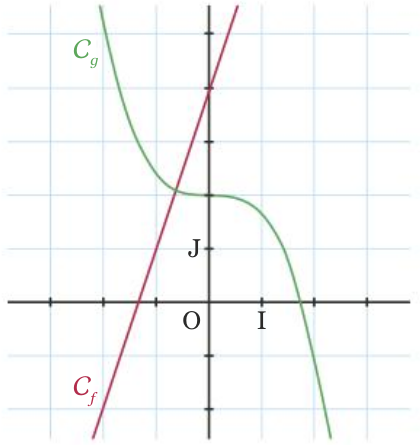
\includegraphics[scale=.3]{courbes2.png}
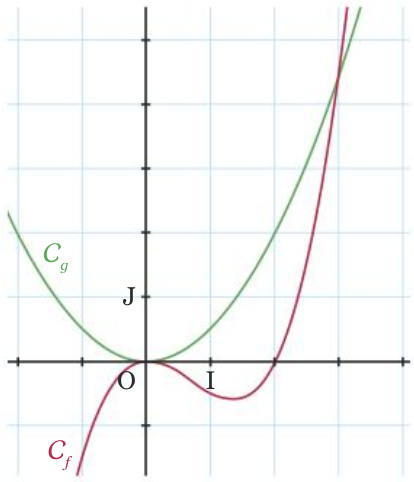
\includegraphics[scale=.3]{courbes1.png}
  \end{center}
\end{minipage}

\paragraph{Exercice 12.}
On considère les fonctions $f$ et $g$ définies sur $\mathbb{R}$ par, pour tout
$x\in\mathbb{R}$, $f(x)=x^2$ et $g(x) = 4x-4$.
\begin{enumerate}
  \item Afficher les représentations graphiques de $f$ et $g$ sur la
    calculatrice.
  \item En appuyant sur la touche \texttt{CALCULS}, puis en sélectionnant
    \texttt{INTERSECTION}, trouver le point d'intersection entre les courbes
    représentatives de $f$ et de $g$.
  \item Vérifier que, pour tout $x\in\mathbb{R}$, $f(x)-g(x)=x^2-4x+4$ puis
    factoriser cette expression.
  \item Donner les solutions de l'équation $f(x)-g(x)=0$.
  \item Quel est le lien entre les questions $1$ et $2$ et les questions $3$ et
    $4$ ?
\end{enumerate}

\paragraph{Exercice 13.}~\\[0mm]
\begin{minipage}{.5\textwidth}
  Associer à chaque tableau de variation ci-dessous la courbe correspondante
  ci-contre.
  \begin{center}
    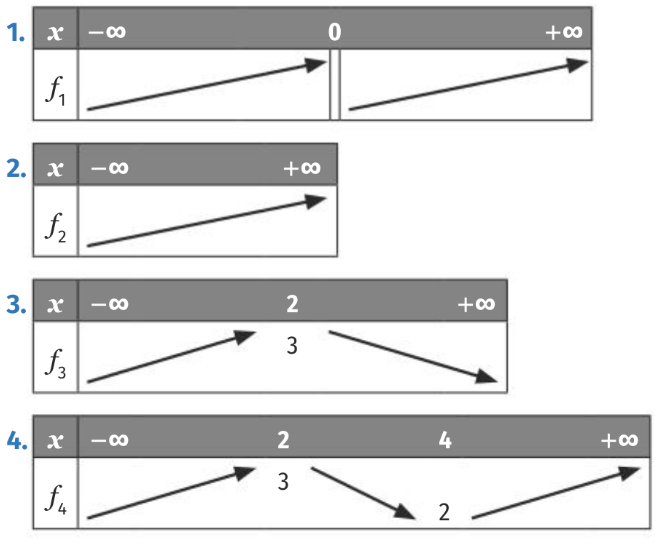
\includegraphics[scale=.3]{tableau.png}
  \end{center}
\end{minipage}
\begin{minipage}{.5\textwidth}
  \begin{center}
    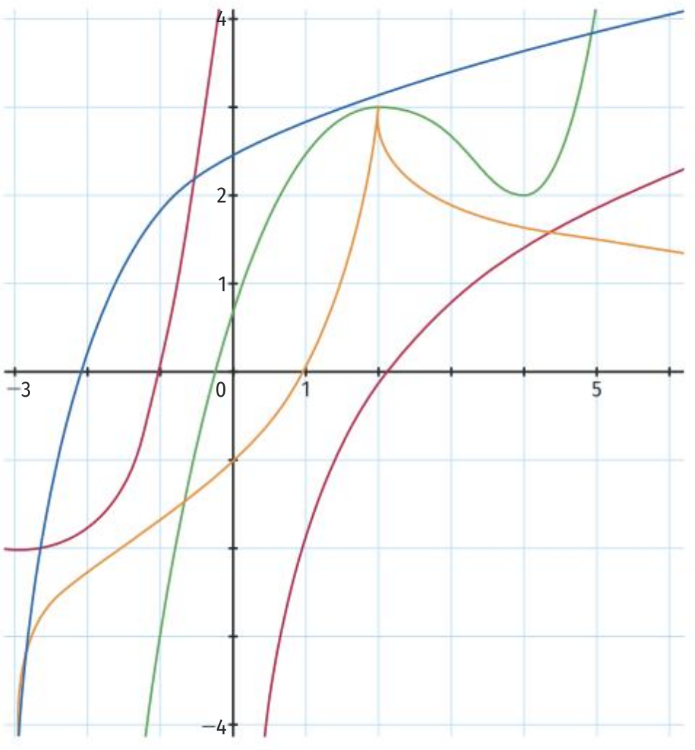
\includegraphics[scale=.26]{4courbes1.png}
  \end{center}
\end{minipage}

\paragraph{Exercice 14.}~\\[-7mm]
\begin{minipage}{.5\textwidth}
  \begin{enumerate}
    \item Pour chaque représentation graphique ci-dessous, desser le tableau de
  variation correspondant.
    \item Préciser si ces courbes admettent un maximum ou un minimum, et le(s)
  donner le cas échéant.
  \end{enumerate}
\end{minipage}
\begin{minipage}{.5\textwidth}
  \begin{center}
    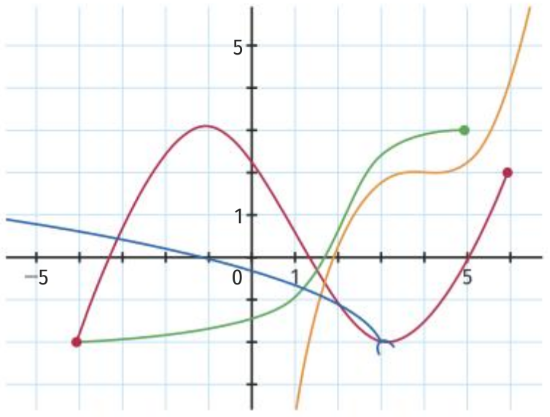
\includegraphics[scale=.3]{4courbes2.png}
  \end{center}
\end{minipage}

\paragraph{Exercice 15.}~\\[1mm]
\begin{minipage}{.5\textwidth}
On considère une fonction $f$ dont le tableau de
variations est donné ci-contre. Répondre par vrai ou par faux aux affirmations
suivantes.
\end{minipage}
\begin{minipage}{.5\textwidth}
  \begin{center}
    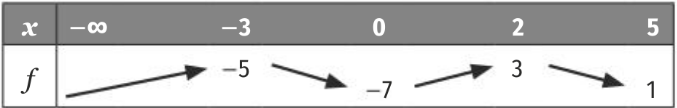
\includegraphics[scale=.3]{tableauvar.png}
  \end{center}
\end{minipage}
~\\[-9mm]
\begin{multicols}{2}
\begin{enumerate}
  \item L'ensemble de définition de $f$ est $[-3;5]$.
  \item $f$ est croissante sur $[-7;3]$
  \item $f$ est d\'ecroissante sur $[-3;2]$
  \item $f$ est d\'ecroissante sur $[2;5]$
  \item $f$ est négative sur $]-\infty;0]$.
  \item $f$ est positive sur $[0;2]$.
  \item $-7$ est le minimum de $f$.
  \item $3$ est le maximum de $f$.
\end{enumerate}
\end{multicols}



\end{document}
